% 6DCIoT 2027 (IEEE PerCom 2027 workshops) submission draft.
% Limit: 6 pages + 1 optional page, IEEE Computer Society format, double-blind.
% Build: latexmk -pdf main.tex   (figures come from testbed/analysis/plot.py into figs/)
% Red [..] = number still to fill from the campaign; blue [TODO ..] = text still to write.
\documentclass[conference,compsoc]{IEEEtran}

\usepackage{cite}
\usepackage{amsmath}
\usepackage{graphicx}
\usepackage{booktabs}
\usepackage{multirow}
\usepackage{xcolor}
\usepackage{url}
\usepackage{tikz}
\usetikzlibrary{positioning,arrows.meta,calc}

\newcommand{\tbd}[1]{\textcolor{red}{[#1]}}
\newcommand{\todo}[1]{\textcolor{blue}{[TODO: #1]}}
% Include a figure if it exists, else a labelled placeholder box of the same width.
\newcommand{\figorbox}[2]{\IfFileExists{#1}{\includegraphics[width=#2]{#1}}%
  {\fbox{\parbox[c][3.2cm][c]{\dimexpr#2-2\fboxsep}{\centering\small Figure pending:\\\texttt{\detokenize{#1}}}}}}

\begin{document}

\title{Link-Level Self-Healing for Container Networks\\at the IoT Edge}

% Double-blind: no names, affiliations, acknowledgements or identifying links.
\author{\IEEEauthorblockN{Anonymous Authors}
\IEEEauthorblockA{Under double-blind review}}

\maketitle

\begin{abstract}
Edge clusters that host IoT services run Kubernetes over links that degrade, flap and
fail independently of the nodes they connect. Kubernetes only notices a failure when a
node stops reporting to the control plane, so a broken path between two healthy nodes
silently blackholes the traffic between them. We present a self-healing pod network
that detects and repairs such faults per node pair. Every node runs two container
networks over separate underlay links, probes every peer on both, and steers traffic
for a broken pair onto the backup network or through a relay node, without changing
any pod or Service address. Node-level failover covers the faults that steering cannot.
On a three-node testbed with an MQTT sensor workload and emulated link cuts, loss,
flapping and CNI faults, stock Kubernetes never recovered during a 60\,s fault, while our
system restored service in a median of \tbd{6.3}\,s, delivered \tbd{100}\% of QoS~1
messages without a single reconnection, and raised availability under 30\% loss from
\tbd{42}\% to \tbd{91}\%. We also report two pitfalls, NAT and reverse-path filtering,
that break connection continuity when paths change under a container network.
\end{abstract}

\begin{IEEEkeywords}
edge computing, Kubernetes, container networking, resilience, IoT, self-healing
\end{IEEEkeywords}

% ======================================================================
\section{Introduction}
\label{sec:intro}

IoT deployments increasingly run their gateways, brokers and analytics as containers
on small Kubernetes clusters at the edge~\cite{burns2016borg,kubeedge}. Unlike a data
centre, the network between edge nodes is heterogeneous and unreliable: nodes are
joined by wired backhaul, Wi-Fi or cellular links that lose packets, flap, or fail
while the nodes themselves stay healthy~\cite{huang2017gray}. For an IoT service the
consequence is concrete: telemetry stops arriving, and messages published at QoS~0 are
lost for good.

Kubernetes does not see these faults. A node is declared \emph{NotReady} only after
its kubelet stops reaching the API server for a grace period (40\,s by default), and
pods are evicted after a further toleration (300\,s by
default)~\cite{k8snodelifecycle}. A broken data path between two worker nodes that
both still reach the control plane is never detected: the Service keeps sending
traffic into the broken path for as long as the fault lasts. Container network
interfaces (CNIs) such as Calico~\cite{calico} and Flannel~\cite{flannel} check their
own agents, not the paths between nodes.

We make the pod network repair itself at the granularity at which edge links fail: a
pair of nodes. Our contributions are:
\begin{itemize}
  \item A \textbf{dual-network design} in which every node runs a primary and a
        backup CNI over separate underlay links, so a pod keeps its address while its
        traffic changes path (Section~\ref{sec:design}).
  \item \textbf{Per-link steering}: all-pairs probing on both networks and a
        per-peer choice of primary, backup, relay through a third node, or an explicit
        \emph{no path} alarm, installed as policy routes, together with node-level
        failover for faults steering cannot repair.
  \item An \textbf{edge testbed and evaluation} with an MQTT sensor workload and six
        fault types, including gray failures, comparing stock Kubernetes, node-level
        failover and our system over \tbd{10} repetitions (Section~\ref{sec:eval}).
  \item Two \textbf{lessons} for any system that changes paths under a container
        network: source NAT and strict reverse-path filtering both silently break
        connections at the moment of a switch (Section~\ref{sec:lessons}).
\end{itemize}
The implementation and testbed are open source.\footnote{Anonymised repository:
\tbd{https://anonymous.4open.science/r/...}}

% ======================================================================
\section{Background and Problem}
\label{sec:background}

\subsection{Pod networking in Kubernetes}
Each pod gets an IP address from the cluster's CNI. Overlay CNIs carry pod traffic
between nodes in a tunnel: Calico encapsulates it in IP-in-IP (IPIP) and Flannel in
VXLAN. Services give a group of pods one virtual address; kube-proxy translates it to
a pod address with destination NAT on the sending node. Multus~\cite{multus} lets a pod
attach to a second CNI as an extra interface.

\subsection{Faults at the edge}
We consider three fault classes that leave both endpoints running:
(i) \emph{link faults} on the underlay between two nodes, from a cut to partial loss
and flapping (gray failures~\cite{huang2017gray});
(ii) \emph{overlay faults}, where the CNI's tunnel between two nodes stops forwarding
while the link works (for example a filtering rule or a broken tunnel endpoint);
(iii) \emph{node CNI faults}, where one node's CNI data plane stops forwarding pod
traffic altogether. Kubernetes detects none of them, because the kubelet's heartbeat to
the API server does not cross the broken pod path.

\subsection{Requirements}
Repair must (R1) act within seconds, (R2) not change pod or Service addresses, so that
open connections such as MQTT sessions survive, (R3) not flap under partial loss,
(R4) never act on missing or stale measurements, and (R5) run on unmodified Kubernetes
and CNIs.

% ======================================================================
\section{Design}
\label{sec:design}

\begin{figure}[t]
\centering
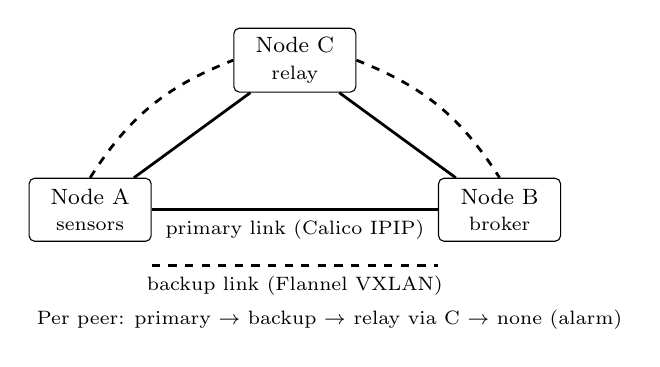
\begin{tikzpicture}[
  node/.style={draw, rounded corners=2pt, minimum width=1.55cm, minimum height=0.8cm,
               align=center, font=\footnotesize},
  prim/.style={line width=1pt},
  back/.style={line width=1pt, dashed},
  flow/.style={-{Stealth[length=2mm]}, line width=0.8pt, gray!70!black}]
  \node[node] (A) at (0,0) {Node A\\\scriptsize sensors};
  \node[node] (B) at (5.2,0) {Node B\\\scriptsize broker};
  \node[node] (C) at (2.6,1.9) {Node C\\\scriptsize relay};
  \draw[prim] (A) -- node[below, font=\scriptsize] {primary link (Calico IPIP)} (B);
  \draw[back] ([yshift=-3mm]A.south east) -- ([yshift=-3mm]B.south west)
     node[midway, below, font=\scriptsize] {backup link (Flannel VXLAN)};
  \draw[prim] (A) -- (C); \draw[prim] (C) -- (B);
  \draw[back] (A.north) to[bend left=18] (C.west);
  \draw[back] (C.east) to[bend left=18] (B.north);
  \node[font=\scriptsize, align=left, anchor=north west] at (-0.8,-1.15)
    {Per peer: primary $\rightarrow$ backup $\rightarrow$ relay via C $\rightarrow$ none (alarm)};
\end{tikzpicture}
\caption{Two pod networks over separate underlay links. When A's primary path to B
fails, A routes B's pod addresses over the backup network, or through C over the
primary network when both direct paths fail.}
\label{fig:arch}
\end{figure}

Figure~\ref{fig:arch} shows the idea. The system has three parts: a health agent and a
link router on every node, and an operator in the control plane.

\subsection{Two networks, one address}
Each node runs Calico as the primary CNI (pod range 172.16.0.0/16) and Flannel as the
backup (10.244.0.0/16), bound to a second underlay interface. Pods receive their
primary address from Calico and, through Multus, a backup interface \emph{net1} from
Flannel. Steering never changes a pod's primary address: it only changes which tunnel
carries packets to the destination node's Calico address block (R2).

\subsection{All-pairs probing}
The health agent on each node probes the agent on every peer, once on its primary and
once on its backup address, every $\Delta$ seconds with a timeout. A path changes state
only after $k$ identical results in a row, which suppresses noise under partial loss
(R3). Each agent publishes its verdicts with a timestamp on its Node object; a report
older than 30\,s is treated as unknown, and unknown never causes a change (R4). On
restart an agent starts from its last report instead of from ``healthy''. With $n$
nodes the agents send $2n(n-1)$ probes per round. Detection therefore takes about
$k\Delta$; we use $\Delta=2$\,s, a 1\,s timeout and $k=3$.

\subsection{Per-link path choice}
The link router on node $A$ reads all reports and chooses, for each peer $B$:
\emph{primary} if $A$'s primary probe to $B$ succeeds; else \emph{backup} if the backup
probe succeeds; else \emph{relay} through a node $C$ whose primary paths $A\to C$ and
$C\to B$ both work; else \emph{none}. A relay, once chosen, is kept while it works,
to avoid oscillating between candidates. The router installs the choice as Linux policy
routing: routes for each of $B$'s Calico address blocks in a dedicated table, pointing
at $B$'s Flannel address on the VXLAN device (backup) or at $C$ on the IPIP device
(relay), and a rule that consults the table before the main one. Probe traffic is
excluded by two higher-priority rules, so the probes keep measuring the real primary
path. The router publishes its choices; the operator aggregates them into the
resource's status, raises a \emph{LinksReachable} condition and emits \emph{NoPath}
and \emph{PathRestored} events. When all probes recover, traffic moves back to the
primary path.

\subsection{Node-level failover}
Steering repairs a path but cannot repair a node whose CNI data plane drops all pod
traffic. For this case the operator, which sees all reports, blames a node only when
probes between other nodes still succeed. It then marks the node's pods unready through
a readiness gate, publishes a ``shadow'' EndpointSlice that points the Service at the
pods' backup addresses, taints the node, and restarts its CNI agent once. Both
mechanisms run together; Section~\ref{sec:eval} measures each.

% ======================================================================
\section{Implementation}
\label{sec:impl}
The system is written in Go \todo{final count: about 1{,}800 lines plus 1{,}800 lines
of tests}: an operator built with controller-runtime, a health-agent DaemonSet and a
link-router DaemonSet that manages routes and rules through netlink. The router needs
only the \texttt{NET\_ADMIN} capability; a short-lived init container sets loose
reverse-path filtering on the two tunnel devices (Section~\ref{sec:lessons}). A
cleanup mode removes every route and rule it owns. All state lives in Kubernetes
objects, so any component can restart at any time without losing or misapplying routes.

% ======================================================================
\section{Evaluation}
\label{sec:eval}

\subsection{Testbed and workload}
We emulate an edge site with three Kubernetes v1.35 nodes (minikube, Docker driver) on
one Linux host (4 cores, 32\,GB). Each node has two interfaces on separate bridged
networks: the primary link carries Calico, the backup link carries Flannel. Node A runs
the clients and node B the services; node C is the control plane and a potential relay.
\begin{itemize}
  \item \textbf{IoT workload:} ten MQTT~\cite{mqtt5} sensors on A, five at QoS~1 and
        five at QoS~0, each publishing 10 messages/s through the Service to a
        Mosquitto broker on B. A subscriber on B timestamps every message.
  \item \textbf{Request workload:} an HTTP prober on A sends 10 requests/s to an
        nginx pod on B, both to its pod address and to its Service, each over a new
        connection with a 500\,ms timeout.
\end{itemize}
All components share one clock, so one-way latencies are exact.

\subsection{Faults and configurations}
Table~\ref{tab:faults} lists the faults. Link faults are injected with \texttt{tc
netem} on the node's interface, only for packets addressed to the peer. We compare
three configurations: \emph{Kubernetes} (no repair), \emph{node failover} only, and
the \emph{full} system; an ablation disables the relay. Each run has 20\,s of normal
traffic, a 60\,s fault and 45\,s of recovery, and every cell is repeated \tbd{10}
times with the fault order rotated.

\begin{table}[t]
\centering
\caption{Fault types (A--B link unless stated)}
\label{tab:faults}
\footnotesize
\begin{tabular}{@{}ll@{}}
\toprule
Fault & Injection \\
\midrule
Link cut & 100\% loss on the primary link \\
Both links cut & 100\% loss on primary and backup links \\
30\% loss & 30\% random loss each way, primary link \\
Flapping & primary link down 5\,s, up 5\,s, repeating \\
Overlay fault & Calico IPIP dropped, link intact \\
Node CNI fault & B drops all forwarded Calico pod traffic \\
\bottomrule
\end{tabular}
\end{table}

\subsection{Recovery time}
\todo{Describe Fig.~\ref{fig:recovery} and Table~\ref{tab:results} from the campaign:
Kubernetes and node failover never recover from link and overlay faults; the full
system recovers in about $k\Delta$; relay adds about 2\,s; node CNI fault is repaired by
node failover in 10--30\,s.}

\begin{figure}[t]
\centering
\figorbox{figs/recovery_cdf_link-cut.pdf}{\columnwidth}\\[2pt]
\figorbox{figs/recovery_bars.pdf}{\columnwidth}
\caption{Service recovery after a primary link cut (top, CDF over \tbd{10} runs) and
median recovery per fault with p95 whiskers (bottom). Runs without recovery are shown
at the fault duration.}
\label{fig:recovery}
\end{figure}

\begin{table}[t]
\centering
\caption{Median recovery time [s] (Service). ``--'': no recovery within 60\,s}
\label{tab:results}
\footnotesize
\begin{tabular}{@{}lccc@{}}
\toprule
Fault & Kubernetes & Node failover & Full system \\
\midrule
Link cut        & \tbd{--} & \tbd{--} & \tbd{6.3} \\
Both links cut  & \tbd{--} & \tbd{--} & \tbd{7.3} \\
Overlay fault   & \tbd{--} & \tbd{--} & \tbd{6.4} \\
Node CNI fault  & \tbd{--} & \tbd{28.7} & \tbd{20.4} \\
\bottomrule
\end{tabular}
\end{table}

\subsection{IoT service continuity}
\todo{Table~\ref{tab:mqtt}: QoS 1 delivery, reconnections and longest gap; QoS 0 loss.
Key point: no MQTT reconnection under steering, because addresses do not change; the
longest gap is the detection time plus TCP's retransmission backoff~\cite{rfc6298}.}

\begin{table}[t]
\centering
\caption{MQTT during a 60\,s primary link cut (median of \tbd{10} runs)}
\label{tab:mqtt}
\footnotesize
\begin{tabular}{@{}lccc@{}}
\toprule
 & Kubernetes & Node failover & Full system \\
\midrule
QoS 0 delivered [\%]   & \tbd{} & \tbd{} & \tbd{100} \\
QoS 1 reconnections    & \tbd{} & \tbd{} & \tbd{0} \\
QoS 1 longest gap [s]  & \tbd{} & \tbd{} & \tbd{6.5} \\
QoS 1 p99 latency [s]  & \tbd{} & \tbd{} & \tbd{} \\
\bottomrule
\end{tabular}
\end{table}

\subsection{Gray failures and flapping}
\todo{Fig.~\ref{fig:avail}: availability under 30\% loss rises from about 42\% to
about 91\% because steering moves the pair off the lossy link and the $k$-streak keeps it
there; flapping faster than $k\Delta$ cannot be helped and does not cause oscillation.}

\begin{figure}[t]
\centering
\figorbox{figs/availability.pdf}{\columnwidth}
\caption{Share of successful Service requests during the fault (median, p5 whisker).}
\label{fig:avail}
\end{figure}

\subsection{Overhead}
\todo{Probe bandwidth and CPU per node; $2n(n-1)$ probes per round; detection time vs.\
probe interval $\Delta\in\{0.5,1,2\}$\,s (M5).}

% ======================================================================
\section{Lessons: Changing Paths Under a Container Network}
\label{sec:lessons}

\textbf{Source NAT ties a connection to an interface.} kube-proxy masquerades Service
traffic whose source lies outside its configured pod range. In our first runs the range
still named the default network, so every Service connection from a primary-network pod
was masqueraded to the address of its outgoing tunnel. Linux discards the NAT state of
a masqueraded connection when its output interface changes, so the next packet left
with a new source address and the broker answered with a reset. Every switch, in both
directions, cost each MQTT client a reconnection and stretched the longest gap from
\tbd{6.5} to \tbd{13}\,s. Configuring kube-proxy with the primary CNI's real pod range
removes the NAT, and with it the resets.

\textbf{Strict reverse-path filtering punishes asymmetry.} Each node switches on its
own probes, so for a few seconds $A\to B$ and $B\to A$ can use different tunnels. With
strict reverse-path filtering, the default on our nodes, each side drops packets that
arrive on the tunnel it would not reply through; under 30\% loss this turned a partial
outage into \tbd{12}\,s of total outage. Loose filtering on the tunnel devices, the
standard setting for multihomed hosts~\cite{rfc3704}, removes the problem.

% ======================================================================
\section{Related Work}
\label{sec:related}

\textbf{Overlay rerouting.} Resilient Overlay Networks~\cite{andersen2001ron} route
around Internet path failures through intermediate overlay nodes, measured by active
probing; our relay applies the same idea inside a container network, without changing
endpoint addresses. IP fast reroute~\cite{rfc5714frr} and BFD~\cite{rfc5880bfd}
provide sub-second detection and precomputed alternates in routers; we bring comparable
per-neighbour detection to Kubernetes nodes, where no routing protocol sees pod paths.

\textbf{Multipath transport.} MPTCP~\cite{rfc8684mptcp} survives path failures when
both endpoints support it and have several addresses; our approach is transparent to
applications and works for any transport.

\textbf{Kubernetes and edge resilience.} Kubernetes handles node failure through
heartbeats and eviction~\cite{k8snodelifecycle}. Service meshes detect failing
endpoints at layer~7 (outlier detection~\cite{istiooutlier}) but can only avoid an
endpoint, not repair the path to it. Multi-cluster fabrics such as
Submariner~\cite{submariner} and Liqo~\cite{iorio2023liqo} connect clusters, and
CEFIoT~\cite{javed2018cefiot} makes IoT processing fault-tolerant through replication
across edge and cloud. \todo{Add 2--3 recent edge-Kubernetes resilience papers,
including any PerCom/6DCIoT work; verify every reference.}

% ======================================================================
\section{Limitations and Future Work}
\label{sec:limits}
\begin{itemize}
  \item \textbf{Binary path state.} A path is up or down; under partial loss we switch
        only after $k$ failed probes in a row. A quality score from probe loss and
        delay would handle gray failures better.
  \item \textbf{Emulated testbed.} All nodes share one host and clock; a deployment on
        heterogeneous edge hardware (for example Raspberry Pi nodes with Wi-Fi and
        cellular uplinks) is future work.
  \item \textbf{Scale.} Probing grows as $n(n-1)$; larger sites need sampled or
        hierarchical probing.
  \item \textbf{One relay hop}, IPv4 only, and the probe port is never steered.
\end{itemize}

% ======================================================================
\section{Conclusion}
\label{sec:conclusion}
\todo{Three sentences: problem, mechanism, headline numbers.}

\bibliographystyle{IEEEtran}
\bibliography{refs}

\end{document}
